% Options for packages loaded elsewhere
\PassOptionsToPackage{unicode}{hyperref}
\PassOptionsToPackage{hyphens}{url}
%
\documentclass[
]{article}
\usepackage{amsmath,amssymb}
\usepackage{iftex}
\ifPDFTeX
  \usepackage[T1]{fontenc}
  \usepackage[utf8]{inputenc}
  \usepackage{textcomp} % provide euro and other symbols
\else % if luatex or xetex
  \usepackage{unicode-math} % this also loads fontspec
  \defaultfontfeatures{Scale=MatchLowercase}
  \defaultfontfeatures[\rmfamily]{Ligatures=TeX,Scale=1}
\fi
\usepackage{lmodern}
\ifPDFTeX\else
  % xetex/luatex font selection
\fi
% Use upquote if available, for straight quotes in verbatim environments
\IfFileExists{upquote.sty}{\usepackage{upquote}}{}
\IfFileExists{microtype.sty}{% use microtype if available
  \usepackage[]{microtype}
  \UseMicrotypeSet[protrusion]{basicmath} % disable protrusion for tt fonts
}{}
\makeatletter
\@ifundefined{KOMAClassName}{% if non-KOMA class
  \IfFileExists{parskip.sty}{%
    \usepackage{parskip}
  }{% else
    \setlength{\parindent}{0pt}
    \setlength{\parskip}{6pt plus 2pt minus 1pt}}
}{% if KOMA class
  \KOMAoptions{parskip=half}}
\makeatother
\usepackage{xcolor}
\usepackage[margin=1in]{geometry}
\usepackage{graphicx}
\makeatletter
\def\maxwidth{\ifdim\Gin@nat@width>\linewidth\linewidth\else\Gin@nat@width\fi}
\def\maxheight{\ifdim\Gin@nat@height>\textheight\textheight\else\Gin@nat@height\fi}
\makeatother
% Scale images if necessary, so that they will not overflow the page
% margins by default, and it is still possible to overwrite the defaults
% using explicit options in \includegraphics[width, height, ...]{}
\setkeys{Gin}{width=\maxwidth,height=\maxheight,keepaspectratio}
% Set default figure placement to htbp
\makeatletter
\def\fps@figure{htbp}
\makeatother
\setlength{\emergencystretch}{3em} % prevent overfull lines
\providecommand{\tightlist}{%
  \setlength{\itemsep}{0pt}\setlength{\parskip}{0pt}}
\setcounter{secnumdepth}{-\maxdimen} % remove section numbering
\usepackage{booktabs}
\usepackage{longtable}
\usepackage{array}
\usepackage{multirow}
\usepackage{wrapfig}
\usepackage{float}
\usepackage{colortbl}
\usepackage{pdflscape}
\usepackage{tabu}
\usepackage{threeparttable}
\usepackage{threeparttablex}
\usepackage[normalem]{ulem}
\usepackage{makecell}
\usepackage{xcolor}
\ifLuaTeX
  \usepackage{selnolig}  % disable illegal ligatures
\fi
\usepackage{bookmark}
\IfFileExists{xurl.sty}{\usepackage{xurl}}{} % add URL line breaks if available
\urlstyle{same}
\hypersetup{
  pdftitle={Article 12 (Salary Schedule) Data},
  pdfauthor={Melissa Anderson, Ph.D.},
  hidelinks,
  pdfcreator={LaTeX via pandoc}}

\title{Article 12 (Salary Schedule) Data}
\author{Melissa Anderson, Ph.D.}
\date{2024-07-25}

\begin{document}
\maketitle

\section{PCC full-time salaries are low compared to neighboring
districts}\label{pcc-full-time-salaries-are-low-compared-to-neighboring-districts}

\begin{verbatim}
## Warning in latex_new_row_builder(target_row, table_info, bold, italic,
## monospace, : Setting full_width = TRUE will turn the table into a tabu
## environment where colors are not really easily configable with this package.
## Please consider turn off full_width.
## Warning in latex_new_row_builder(target_row, table_info, bold, italic,
## monospace, : Setting full_width = TRUE will turn the table into a tabu
## environment where colors are not really easily configable with this package.
## Please consider turn off full_width.
\end{verbatim}

\begin{table}[left]
\centering
\caption{\label{tab:unnamed-chunk-1}Table 2: Area CCC District Representive Salaries During the 2023-204 Academic Year Before and After Adjustment for Local Cost of Living}
\centering
\begin{tabu} to \linewidth {>{\raggedright}X>{\raggedleft}X>{\raggedleft}X}
\hline
District & Aggregate Salary & Adjusted Aggregate Salary\\
\hline
Cerritos & \$128,344 & \$134,674\\
\hline
Santa Clarita & \$124,483 & \$127,283\\
\hline
El Camino & \$121,875 & \$127,086\\
\hline
Long Beach & \$117,589 & \$122,616\\
\hline
Rio Hondo & \$117,057 & \$120,429\\
\hline
Los Angeles & \$118,500 & \$118,500\\
\hline
Santa Monica2 & \$113,300 & \$113,413\\
\hline
\cellcolor[HTML]{9c1521}{\textcolor{white}{\textbf{Pasadena Area}}} & \cellcolor[HTML]{9c1521}{\textcolor{white}{\textbf{\$112,095}}} & \cellcolor[HTML]{9c1521}{\textcolor{white}{\textbf{\$112,095}}}\\
\hline
Glendale & \$103,001 & \$103,001\\
\hline
Compton & \$87,185 & \$90,912\\
\hline
\end{tabu}
\end{table}

\begin{itemize}
\tightlist
\item
  Aggregate Salary is composite value made by averaging values for the
  five representative salary steps found in the CFT Salary Report.
  \emph{(Data Source:
  \url{https://www.cft.org/faculty-salary-comparisons})}
\end{itemize}

\section{PCC full-time salaries have not significantly increased
relative to
inflation}\label{pcc-full-time-salaries-have-not-significantly-increased-relative-to-inflation}

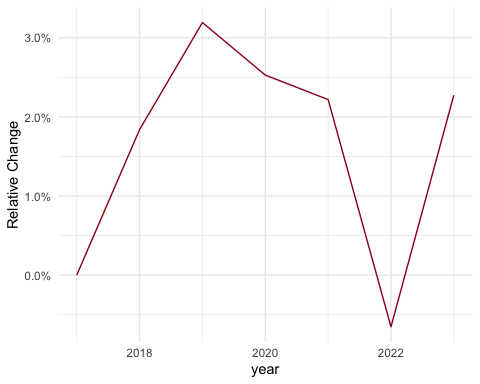
\includegraphics{salary_argument_files/figure-latex/unnamed-chunk-2-1.pdf}

\textbf{Figure 1:} Relative Changes in Aggregate Salary of Full-Time PCC
Faculty since 2017. Aggregate Salary is composite value made by
averaging values for the five representative salary steps found in the
CFT Salary Report. (Data Source:
\url{https://www.cft.org/faculty-salary-comparisons})

\section{The District has seen a significant increase in income relative
to expenses and total
compensation}\label{the-district-has-seen-a-significant-increase-in-income-relative-to-expenses-and-total-compensation}

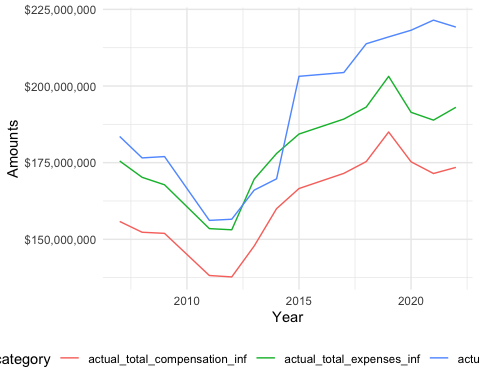
\includegraphics{salary_argument_files/figure-latex/budget_time_plot-1.pdf}

\textbf{Figure 2:} Total Income, Expenses and Compensation Expenses over
time. Values have been adjusted to 2024 dollars to remove the effect of
inflation. \emph{(Data Source:
\url{https://pasadena.edu/business-administrative-services/fiscal-services/budget-forecast-analysis.php})}

\section{Extra funds could be used for a significant increase to total
compensation}\label{extra-funds-could-be-used-for-a-significant-increase-to-total-compensation}

\begin{table}[left]
\centering
\caption{\label{tab:how_much_is_left}Table 1: Non-Expense Income and Amounts Left Over After Expenses are Deducted (2024 Dollars)}
\centering
\begin{tabu} to \linewidth {>{\raggedleft}X>{\raggedleft}X>{\raggedleft}X>{\raggedleft}X>{\raggedleft}X}
\hline
Year & Total Left & \% of Total Expenses & Minus Raise A* & Minus Raise B*\\
\hline
2007 & \$8,000,202 & 4.6\% & -4.3\% & 0.1\%\\
\hline
2008 & \$6,330,784 & 3.7\% & -5.2\% & -0.8\%\\
\hline
2009 & \$9,199,920 & 5.5\% & -3.6\% & 1.0\%\\
\hline
2011 & \$2,689,235 & 1.8\% & -7.3\% & -2.7\%\\
\hline
2012 & \$3,442,679 & 2.2\% & -6.7\% & -2.2\%\\
\hline
2013 & \$-3,581,440 & -2.1\% & -10.8\% & -6.5\%\\
\hline
2014 & \$-8,268,652 & -4.6\% & -13.6\% & -9.1\%\\
\hline
2015 & \$18,827,935 & 10.2\% & 1.2\% & 5.7\%\\
\hline
2017 & \$15,181,786 & 8.0\% & -1.0\% & 3.5\%\\
\hline
2018 & \$20,640,920 & 10.7\% & 1.6\% & 6.1\%\\
\hline
2019 & \$12,871,741 & 6.3\% & -2.8\% & 1.8\%\\
\hline
2020 & \$26,762,033 & 14.0\% & 4.8\% & 9.4\%\\
\hline
2021 & \$32,611,657 & 17.3\% & 8.2\% & 12.7\%\\
\hline
2022 & \$26,163,564 & 13.6\% & 4.6\% & 9.1\%\\
\hline
\end{tabu}
\end{table}

\begin{itemize}
\tightlist
\item
  Percentage of Total Expenses (i.e.~``Reserve'') Left after a (A) 10\%
  or (B) 5\% Increase in Total Compensation. \emph{(Data Source:
  \url{https://pasadena.edu/business-administrative-services/fiscal-services/budget-forecast-analysis.php})}
\end{itemize}

\section{Useful Links}\label{useful-links}

\begin{itemize}
\tightlist
\item
  \emph{Update on community college reserves.}
  \url{https://lao.ca.gov/Publications/Report/4323}. (January 27, 2021)
\item
  \emph{Faculty salary comparison studies. CFT -- a Union of Educators
  and Classified Professionals.}
  \url{https://www.cft.org/faculty-salary-comparisons}.
\item
  \emph{Budget / Forecast \& Analysis - Business and Administrative
  Services - Pasadena City College.}
  \url{https://pasadena.edu/business-administrative-services/fiscal-services/budget-forecast-analysis.php}.
\end{itemize}

\end{document}
